\documentclass[]{article}
\usepackage{lmodern}
\usepackage{amssymb,amsmath}
\usepackage{ifxetex,ifluatex}
\usepackage{fixltx2e} % provides \textsubscript
\ifnum 0\ifxetex 1\fi\ifluatex 1\fi=0 % if pdftex
  \usepackage[T1]{fontenc}
  \usepackage[utf8]{inputenc}
\else % if luatex or xelatex
  \ifxetex
    \usepackage{mathspec}
  \else
    \usepackage{fontspec}
  \fi
  \defaultfontfeatures{Ligatures=TeX,Scale=MatchLowercase}
\fi
% use upquote if available, for straight quotes in verbatim environments
\IfFileExists{upquote.sty}{\usepackage{upquote}}{}
% use microtype if available
\IfFileExists{microtype.sty}{%
\usepackage{microtype}
\UseMicrotypeSet[protrusion]{basicmath} % disable protrusion for tt fonts
}{}
\usepackage[unicode=true]{hyperref}
\hypersetup{
            pdftitle={ ISOQuant 1.6 Help pages},
            pdfauthor={Jörg Kuharev, Pedro Navarro and Stefan Tenzer},
            pdfborder={0 0 0},
            breaklinks=true}
\urlstyle{same}  % don't use monospace font for urls
\usepackage{listings}
\usepackage{longtable,booktabs}
\usepackage{graphicx,grffile}
\makeatletter
\def\maxwidth{\ifdim\Gin@nat@width>\linewidth\linewidth\else\Gin@nat@width\fi}
\def\maxheight{\ifdim\Gin@nat@height>\textheight\textheight\else\Gin@nat@height\fi}
\makeatother
% Scale images if necessary, so that they will not overflow the page
% margins by default, and it is still possible to overwrite the defaults
% using explicit options in \includegraphics[width, height, ...]{}
\setkeys{Gin}{width=\maxwidth,height=\maxheight,keepaspectratio}
\IfFileExists{parskip.sty}{%
\usepackage{parskip}
}{% else
\setlength{\parindent}{0pt}
\setlength{\parskip}{6pt plus 2pt minus 1pt}
}
\setlength{\emergencystretch}{3em}  % prevent overfull lines
\providecommand{\tightlist}{%
  \setlength{\itemsep}{0pt}\setlength{\parskip}{0pt}}
\setcounter{secnumdepth}{5}
% Redefines (sub)paragraphs to behave more like sections
\ifx\paragraph\undefined\else
\let\oldparagraph\paragraph
\renewcommand{\paragraph}[1]{\oldparagraph{#1}\mbox{}}
\fi
\ifx\subparagraph\undefined\else
\let\oldsubparagraph\subparagraph
\renewcommand{\subparagraph}[1]{\oldsubparagraph{#1}\mbox{}}
\fi
\usepackage[left=2cm,right=1.5cm,top=1.5cm,bottom=1.5cm]{geometry}
% \setlength{\parindent}{0.25in}
\setlength{\parskip}{0.4cm}
\pagestyle{plain}

\usepackage[utf8]{inputenc}

\lstset{literate=%
    {Ö}{{\"O}}1
    {Ä}{{\"A}}1
    {Ü}{{\"U}}1
    {ß}{{\ss}}1
    {ü}{{\"u}}1
    {ä}{{\"a}}1
    {ö}{{\"o}}1
    {~}{{\textasciitilde}}1
}

\renewcommand{\contentsname}{Table of contents}

\usepackage{color}
% \definecolor{bgColor}{rgb}{1,1,0.95}
% \pagecolor{bgColor}

\definecolor{middlegray}{rgb}{0.5,0.5,0.5}
\definecolor{lightgray}{rgb}{0.8,0.8,0.8}
\definecolor{orange}{rgb}{0.8,0.3,0.3}
\definecolor{yac}{rgb}{0.6,0.6,0.1}
% settings for lstlisting environment
\lstset{
  basicstyle=\small\ttfamily,
  keywordstyle=\bfseries\ttfamily\color{orange},
  stringstyle=\color{black}\ttfamily,
  commentstyle=\color{middlegray}\ttfamily,
  emph={square}, 
  emphstyle=\color{blue}\texttt,
  emph={[2]root,base},
  emphstyle={[2]\color{yac}\texttt},
  showstringspaces=false,
  flexiblecolumns=false,
  tabsize=2,
%  numbers=left,
%  numberstyle=\tiny,
%  numberblanklines=false,
%  stepnumber=1,
%  numbersep=10pt,
  language=sh, 
  numbers=none,
  frame=shadowbox,
  xleftmargin=15pt,
  backgroundcolor={\color{lightgray}},
  texcl=\true,
  extendedchars=\true
}

\renewcommand{\baselinestretch}{1.0}\normalsize

\title{\texttt{\vspace{4cm}}\\
ISOQuant 1.6\\
\textbf{Help pages}}
\author{Jörg Kuharev, Pedro Navarro and Stefan Tenzer}
\date{\today \thispagestyle{empty}\\
\textbf{NOTE:}\\
Some contents of this document are not\\
aligned with the current software version.\\
An update is coming soon \ldots{} \clearpage}

\begin{document}
\maketitle

{
\setcounter{tocdepth}{3}
\tableofcontents
}
\clearpage

\renewcommand{\baselinestretch}{1.0}

\normalsize

\section{Description}\label{description}

ISOQuant is an academically developed, integrated bioinformatics
pipeline for in-depth evaluation and statistical data analysis of
data-independent acquisition (MS\textsuperscript{E} and
IMS-MS\textsuperscript{E}) based label-free quantitative proteomics that
improves data reliability and quality by application of well-established
and novel analysis methods.

\subsection{About ISOQuant}\label{about-isoquant}

One of the main bottlenecks in the evaluation of label-free quantitative
proteomics experiments is the often cumbersome data export for in-depth
data evaluation and analysis. Data-independent, alternate scanning LC-MS
(MS\textsuperscript{E}/HDMS\textsuperscript{E}/UDMS\textsuperscript{E})
peptide fragmentation data can currently only be processed by Waters
PLGS software (and by recently introduced Progenesis QI for Proteomics
(Nonlineare Dynamics / Waters)).\\
PLGS performs absolute quantification only on a run-to-run level, it
does not afford absolute quantification of protein isoforms and
label-free relative quantification of peptides and proteins based on
clustered accurate mass-retention time pairs on a complete experiment
basis.\\
The bioinformatics pipeline ISOQuant directly accesses xml files from
the PLGS root folder and browses for relevant data from a label-free
Expression Analysis project (quantification analyses, sample
descriptions, search results) for fully automated import into a MySQL
database. EMRTs are subjected to multidimensional LOWESS-based intensity
normalization and annotated by matching exact masses and aligned
retention times of detected features with highest scoring peptide
identification data from associated workflows. Based on the annotated
cluster table, ISOQuant calculates absolute in-sample amounts with an
integrated protein isoform quantification method, utilizing average
intensities of proteotypic peptides for the partitioning of non-unique
peptide intensities between protein isoforms. All data is stored in a
local MySQL based database that can be queried directly by experienced
users.

\subsection{Citing ISOQuant}\label{citing-isoquant}

ISOQuant has been developed since 2009. We introduced the basic
principles of ISOQuant analysis to the community as part of a Nature
Methods articles 2014 (Distler et al. 2014).

\begin{lstlisting}
Distler, U., Kuharev, J., Navarro, P., Levin, Y., Schild, H., & Tenzer, S.
(2014). Drift time-specific collision energies enable deep-coverage
data-independent acquisition proteomics. 
Nature Methods, 11(2), 167–170. http://doi.org/10.1038/nmeth.2767
\end{lstlisting}

Please cite the mentioned publication, when using ISOQuant to produce
publication data or referencing to ISOQuant in other context. Use the
following BibTeX code to import into the reference manager of your
choice:

\begin{lstlisting}
@article{distler_drift_2014,
    title = {Drift time-specific collision energies enable 
        deep-coverage data-independent acquisition proteomics},
    author = {Distler, Ute and Kuharev, Jörg and Navarro, Pedro
        and Levin, Yishai and Schild, Hansjörg and Tenzer, Stefan},
    journal = {Nature Methods},
    volume = {11},
    issn = {1548-7091},
    url = {http://www.nature.com/nmeth/journal/v11/n2/full/nmeth.2767.html},
    doi = {10.1038/nmeth.2767},
    month = feb,
    year = {2014},
    pages = {167--170}
}
\end{lstlisting}

\clearpage

\subsection{ISOQuant workflow}\label{isoquant-workflow}

The data analysis workflow (see fig. \ref{pic:iqWorkflow}) consists of
raw data preprocessing using vendor software PLGS and the downstream
analysis using ISOQuant. In our data analysis workflow, PLGS is used for
the initial signal processing as well as for peptide and protein
identification. Before automatically importing PLGS results into a
relational database (MySQL), ISOQuant allows to change the structure of
underlying PLGS project and in this way to redesign the label-free
experiment. The ISOQuant data analysis workflow is composed of multiple
dedicated algorithms. At different stages of analysis, data is filtered
on peptide and protein level based on user defined criteria
(identification score and type, sequence length, replication rate, FDR
threshold, etc.) to ensure a constant level of high data quality for all
runs in the project. The retention time alignment procedure corrects
non-linear retention time distortions between LC-MS runs of the
experiment (Podwojski et al. 2009). To group corresponding features from
different runs of the experiment, exact mass and retention time pairs
(EMRT) extended by ion mobility values are evaluated using the density
based clustering algorithm DBSCAN (Ester et al. 1996). Resulting feature
clusters are annotated by evaluation of consent peptide identifications
and identification probabilities. The feature cluster annotation
approach transfers peptide identifications between runs and reduces
missing values increasing the reproducibility of data analysis.
Resolving ambiguous peptides-in-proteins networks, the protein homology
filtering algorithm reduces side effects of the protein inference
problem (Nesvizhskii and Aebersold 2005). The multi-dimensional feature
intensity normalization algorithm reduces the effects of technical
variance between independently acquired LC-MS runs of the experiment and
increases the reproducibility of quantification. Finally, ISOQuant uses
a derivative of the Top3 method (Silva et al. 2006) for the absolute
protein quantification and exports analysis results to multiple output
formats for subsequent interpretation. Alternatively to ISOQuant, the
commercial software Progenesis QI for proteomics (Nonlinear Dynamics /
Waters) or the freely available R-package synapter (Bond et al. 2013)
could also be used to analyze MS\textsuperscript{E} data. In a recent
study, we tested Progenesis QIP, synapter and ISOQuant for the
performance of protein identification and the label-free quantification
based on the analysis a complex metaproteome sample set (Kuharev et al.
2015).

\begin{figure}[htbp]
\centering
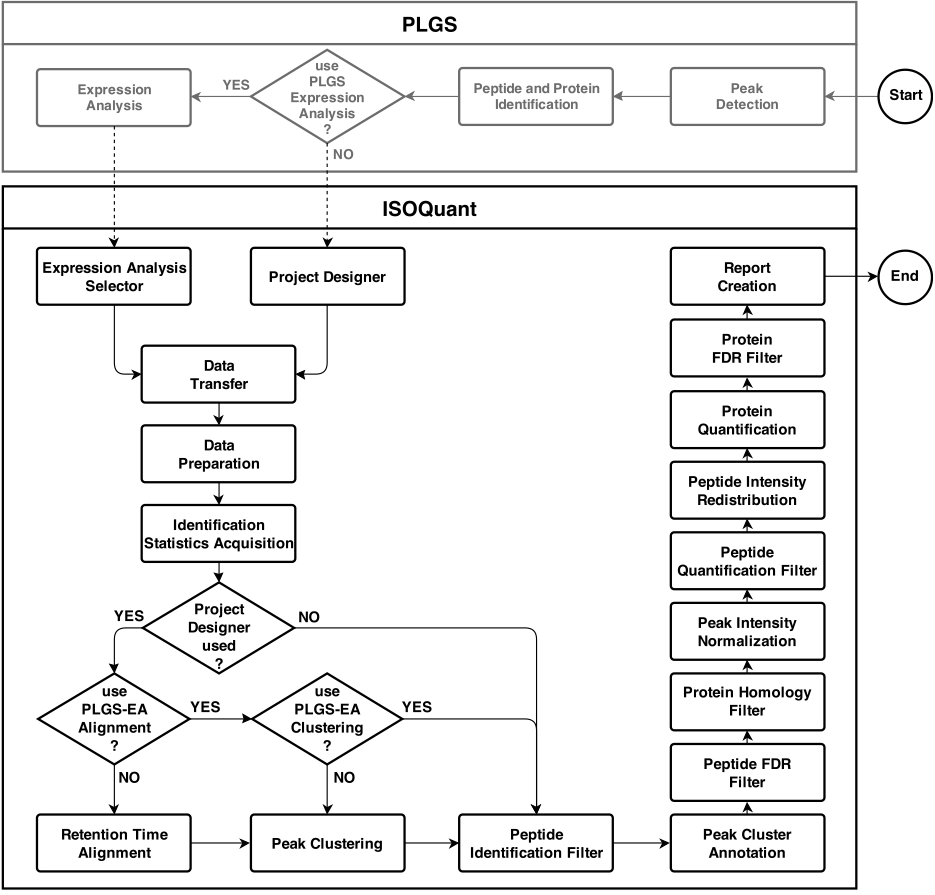
\includegraphics{pic/isoquant_workflow.png}
\caption{The workflow of ISOQuant analysis \label{pic:iqWorkflow}}
\end{figure}

\clearpage

\subsection{Known problems}\label{known-problems}

\begin{itemize}
\tightlist
\item
  On some \textbf{Windows Vista} or \textbf{Window 7} machines ISOQuant
  can not write its configuration file. In this case you have to execute
  ISOQuant with administrative privileges or correct file system
  permissions for ISOQuant installation folder. This is not an ISOQuant
  issue, sometimes Windows messes up file system permissions by using
  different and inconsistent user privileges at different time points.
\item
  Analysis of high complexity datasets may take a while.
\item
  Importing (and analyzing) large projects or runs of high complexity
  may cause out of memory errors, make sure your PC has enough memory
  and assign more Heap-Space to Java Virtual Machine for running
  ISOQuant Application.
\item
  ISOQuant may fail to import and process data if some PLGS project
  files are broken.
\item
  Running MySQL on Mac OSX machines significantly decreases the
  performance of ISOQuant. This is a known problem of MySQL not of
  ISOQuant. Use Windows or Linux machines and/or install MariaDB instead
  of MySQL for better performance.
\end{itemize}

\clearpage

\section{Program requirements}\label{program-requirements}

ISOQuant will only work properly if the system for running ISOQuant
meets following requirements.

\begin{itemize}
\item
  Operating System: Windows, Mac OS X or Linux
\item
  PLGS root folder with projects containing processed
  MS\textsuperscript{E}/HDMS\textsuperscript{E}/UDMS\textsuperscript{E}
  data is accessible (tested PLGS versions: 2.3/2.4/2.5/3.0)
\item
  at least 3GB RAM
\item
  Java Runtime Environment version 1.6.0 (or newer) is installed and
  works properly
\item
  MySQL Server 5.1 (or newer) is installed and running on local machine
  or network. (tested MySQL versions: 5.1 - 5.5)
\item
  MySQL configuration file options for heap and temporary tables have
  large values as shown in following listing. In some cases it may be
  useful also to increase the size of MySQL thread stack.

\begin{lstlisting}
max_heap_table_size = 2048M
tmp_table_size = 2048M
thread_stack = 256K
\end{lstlisting}

  Depending on your operating system and MySQL-Version the configuration
  file is named either my.ini or my.cnf and its location may vary.

  Following listing shows an example of MySQL configuration section
  {[}mysqld{]} working for us on MacOSX 10.6.8 Snow Leopard running
  MySQL Server from XAMPP 1.7.3, the configuration file is located in
  \lstinline!/Applications/XAMPP/xamppfiles/etc/my.cnf!

\begin{lstlisting}
[mysqld]
port = 3306
socket = /Applications/XAMPP/xamppfiles/var/mysql/mysql.sock
skip-locking
key_buffer = 128M
max_allowed_packet = 16M
table_cache = 128
sort_buffer_size = 32M
read_buffer_size = 8M
read_rnd_buffer_size = 8M
net_buffer_length = 64K
thread_stack = 256K
myisam_sort_buffer_size = 32M
tmpdir = /Applications/XAMPP/xamppfiles/temp/
max_heap_table_size = 2048M
tmp_table_size = 2048M
sync_frm = 0
skip-sync-frm=OFF
\end{lstlisting}

  Do not forget to restart MySQL after editing its configuration!
\end{itemize}

Expert note:\\
If you get some ``out of memory'' errors while running ISOQuant please
make sure you start the application by giving Java Virtual Machine a
chance to have enough memory space by command line options, e.g.

\begin{lstlisting}
java -Xms256m -Xmx2G -jar ISOQuant.jar
\end{lstlisting}

this command will assign up to 2 GBs (parameter \textbf{-Xmx2G}) RAM to
the virtual machine and run the ISOQuant application. For some very
complex datasets, it may be useful to increase the \textbf{-Xmx} value
e.g. \textbf{-Xmx48G} to allow the virtual machine to access 48 GBs of
RAM.

\clearpage

\section{Data requirements}\label{data-requirements}

\subsection{Rawdata type}\label{rawdata-type}

ISOQuant has been developed for Waters QTOF LC-MSE and Waters Synapt
G2/G2-S
LC-MS\textsuperscript{E}/HDMS\textsuperscript{E}/UDMS\textsuperscript{E}
instrument data. At this time, only 1D-UPLC data is fully supported,
2D-UPLC support will be included in later releases.

\subsection{Database searches}\label{database-searches}

At the moment, ISOQuant can only process Ion Accounting workflows
(MS\textsuperscript{E}/HDMS\textsuperscript{E}/UDMS\textsuperscript{E}-data).
Classical DDA-Type experiments are not yet supported.

\subsection{Project design}\label{project-design}

There are two different ways to use ISOQuant either as an extension to
PLGS Expression Analysis or completely replacing it.

\subsubsection{Expression analysis}\label{expression-analysis}

You can use your experiment design given by running PLGS Expression
analysis. As a prerequisite for this approach, a complete expression
analysis of multiple samples and replicates is required. In PLGS, please
select autonormalization of samples for generating EMRT and protein
tables. Both EMRT and Protein tables have to be created during the
expression analysis. Each expression analysis within a PLGS project can
be selected during processing in ISOQuant. ISOQuant will create separate
databases for storing the data of every single processed expression
analysis.

\subsubsection{ISOQuant Project
Designer}\label{isoquant-project-designer}

As an alternative to the PLGS Expression analysis, you can use the
simple and efficient built-in Project Designer described in section
\ref{sec:ProjectDesigner}.

\subsection{Peak
detection/alignment/clustering}\label{peak-detectionalignmentclustering}

ISOQuant is based on peak detection, alignment and clustering of data
performed by PLGS. We are aware of some peak
splitting/alignment/clustering issues in PLGS. Therefore, we have have
spent a lot of time to develop own methods for these tasks. You can
either keep EMRT alignment/clustering results or let ISOQuant do the
complete analysis. For details see future publications.

\clearpage

\section{GUI and control elements}\label{gui-and-control-elements}

\subsection{Main view}\label{main-view}

Figure \ref{pic:mainView} shows the main view of ISOQuant. User
interaction is applied by following control elements:

\begin{enumerate}
\def\labelenumi{\arabic{enumi}.}
\tightlist
\item
  List of projects found in PLGS root folder
\item
  List of projects from ISOQuant database
\item
  Button choose PLGS root folder
\item
  Button choose database
\item
  Button restore project from file
\item
  Button find projects
\item
  Button edit configuration
\item
  Button show help window
\item
  Button shutdown application
\end{enumerate}

\begin{figure}[htbp]
\centering
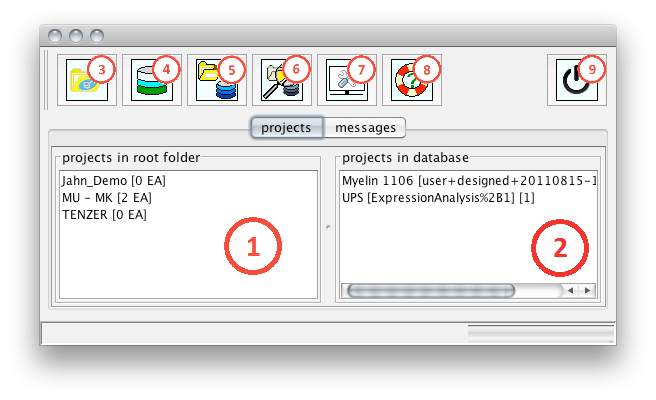
\includegraphics{pic/gui.png}
\caption{the main view of ISOQuant \label{pic:mainView}}
\end{figure}

\clearpage

\subsection{Project Finder}\label{project-finder}

The Project Finder window as shown in figure \ref{pic:FinderWindow}
makes possible to search projects lists for projects by substrings of
project titles and regular expressions matching to them. In case your
search string matches to one or multiple projects the Project Finder
will mark these projects by selecting them in both file system and
database projects lists. The Project Finder window can be accessed by
clicking the button find projects from the tool bar on the main
application window.

\begin{figure}[htbp]
\centering
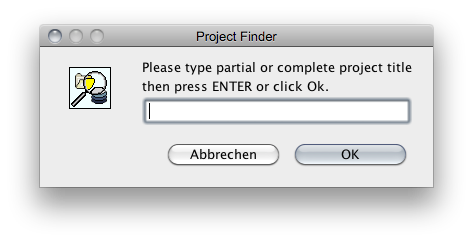
\includegraphics{pic/project_finder.png}
\caption{Project Finder window \label{pic:FinderWindow}}
\end{figure}

\clearpage

\subsection{Context menu for PLGS projects in file
system}\label{context-menu-for-plgs-projects-in-file-system}

Advanced options for each project from PLGS root folder are available
from a context menu like shown in figure \ref{pic:FSContextMenu}:

\begin{enumerate}
\def\labelenumi{\arabic{enumi}.}
\tightlist
\item
  find in database\\
  finds selected projects in the list of projects from database by
  comparing their titles and select them if such projects exist.
\item
  about project\\
  shows additional information about selected projects.
\item
  import and process\\
  allows to select one of predefined processing queues and starts
  processing selected projects using selected processing queue.
\end{enumerate}

\begin{figure}[htbp]
\centering
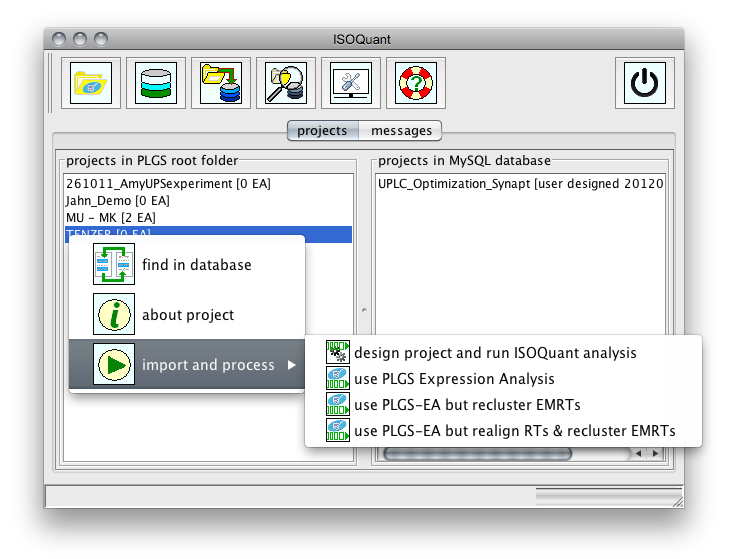
\includegraphics{pic/fs_context.png}
\caption{Context menu for PLGS projects in file system
\label{pic:FSContextMenu}}
\end{figure}

\clearpage

\subsection{Context menu for projects in
database}\label{context-menu-for-projects-in-database}

Advanced options for each project from database are available from a
context menu like shown in figure \ref{pic:DBContextMenu}

\begin{enumerate}
\def\labelenumi{\arabic{enumi}.}
\tightlist
\item
  find in file system\\
  finds selected projects in the list of projects from file system by
  comparing their titles and select them if such projects exist.
\item
  show info\\
  shows additional information about selected projects.
\item
  rename project\\
  rename selected projects.
\item
  reprocess\\
  reprocess a project starting from user selected processing stage. All
  needed subsequent processing steps are automatically applied.
\item
  create report\\
  generate on of implemented report types.
\item
  export to file\\
  export selected projects from database to (backup) files which can be
  imported by other ISOQuant instances.
\item
  remove from database\\
  removes selected projects from database.
\end{enumerate}

\begin{figure}[htbp]
\centering
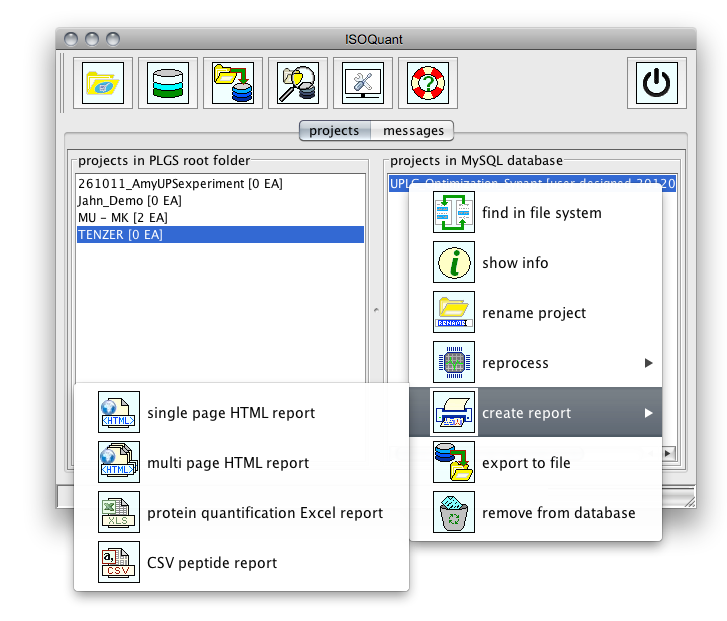
\includegraphics{pic/db_context.png}
\caption{Context menu for already processed projects
\label{pic:DBContextMenu}}
\end{figure}

\textbf{Note:} We continue to develop and improve ISOQuant. The context
menus could look different in different software releases. The elements
in context menus are subject of change, their number and order may vary.

\clearpage

\subsection{Expression Analysis
Selector}\label{expression-analysis-selector}

In some cases a single PLGS project contains multiple defined Expression
Analyses. Some processing queues work with project structures provided
by PLGS Expression Analyses. These queues start with the selection of
contained expression analyses for each selected project. The selection
of expression analyses is done within the Expression Analysis Selector
window as shown in figure \ref{pic:EASelector} by activating the
checkboxes from the column include for each Expression Analysis to be
processed. The Expression Analysis Selector shows each previously
selected project in its own tab pane. ISOQuant generates a separate
database for each selected Expression Analysis.

\begin{figure}[htbp]
\centering
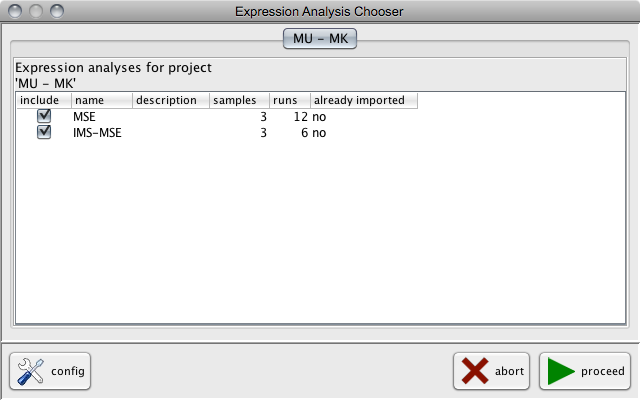
\includegraphics{pic/expression_analysis_selector.png}
\caption{Expression Analysis Selector \label{pic:EASelector}}
\end{figure}

\clearpage

\subsection{\texorpdfstring{Project Designer
\label{sec:ProjectDesigner}}{Project Designer }}\label{project-designer}

ISOQuant allows to create user defined project structures and then to
process these newly structured project data. User defined project
structures are created using the Project Designer as shown in figure
\ref{pic:ProjectDesigner}. The Project Designer window shows the PLGS
project structure on the left and the user defined structure on the
right. A new project structure is created by drag and drop based moving
of workflows, samples or groups between left and right structure trees.
Additionally to drag and drop actions, right click context menus are
available on the right side of Project Designer enabling editing and
removing of selected structure elements. On the top of window you can
switch between Project Designer panes to restructure each previously
selected PLGS project. Processing of designed project can be initiated
by clicking the button Ok on the bottom of window or can be aborted by
clicking the Cancel button. While processing ISOQuant generates a
separate database for each designed project.

\begin{figure}[htbp]
\centering
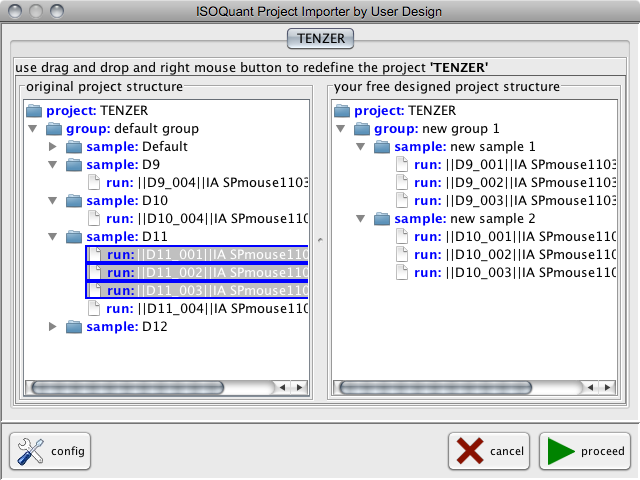
\includegraphics{pic/project_designer.png}
\caption{Project Designer \label{pic:ProjectDesigner}}
\end{figure}

\section{ISOQuant configuration}\label{isoquant-configuration}

ISOQuant stores parameters for program behavior and data processing
algorithms in a single configuration file named \textbf{isoquant.ini}.
This configuration file is located in the folder you have installed
ISOQuant to. For resetting parameters to default values just close
ISOQuant then delete or rename the configuration file (or single
parameter lines) and start ISOQuant again. If no configuration file can
be found on application start a new one will be created using default
parameter values.\\
\textbf{Do not change the configuration file unless you know what you
do!}

ISOQuant configuration can be edited from ISOQuant Configuration Editor
accessible from graphical user interface. Configuration Editor allows to
edit parameters and also export/import configuration settings to/from
files.

Two configuration files are provided with ISOQuant installation
packages:

\begin{itemize}
\tightlist
\item
  \textbf{isoquant\_high\_confidence.ini} example configuration file for
  high confidence quantitative analyses
\item
  \textbf{isoquant\_maxID.ini} example configuration file for discovery
  proteomics experiments
\end{itemize}

These files can be imported into ISOQuant from Configuration Editor or
manually copied to \textbf{isoquant.ini} file.

\clearpage

\section{Configuration guide}\label{configuration-guide}

This chapter lists and describes the main set of available parameters.
The number of parameters, their names and the behavior of application
caused by parameters are subjects of change because we actively work on
improving ISOQuant and underlying methods. Thus the following list of
parameters may be incomplete and/or up to date.

\subsection{EMRT cluster annotation}\label{emrt-cluster-annotation}

\subsubsection{Peptide identification
filter}\label{peptide-identification-filter}

User can define minimum reliability criteria for a peptide to be used
for ISOQuant processing. \emph{Note:} Only peptides passing this filter
will be used for all further analysis steps!

\paragraph{Peptide types}\label{peptide-types}

Peptides identified in first pass of PLGS database search (type:
\textbf{PEP\_FRAG\_1}) are generally accepted. Setting one of following
parameters to TRUE will configure ISOQuant to accept additional peptide
types.

\begin{itemize}
\tightlist
\item
  \textbf{process.identification.peptide.acceptType.IN\_SOURCE}=false
\item
  \textbf{process.identification.peptide.acceptType.MISSING\_CLEAVAGE}=false
\item
  \textbf{process.identification.peptide.acceptType.NEUTRAL\_LOSS\_H20}=false
\item
  \textbf{process.identification.peptide.acceptType.NEUTRAL\_LOSS\_NH3}=false
\item
  \textbf{process.identification.peptide.acceptType.PEP\_FRAG\_2}=false
\item
  \textbf{process.identification.peptide.acceptType.PTM}=false
\item
  \textbf{process.identification.peptide.acceptType.VAR\_MOD}=false
\end{itemize}

Following additional filtering criteria are used as thresholds to select
peptides used for further processing steps.

\begin{itemize}
\tightlist
\item
  \textbf{process.identification.peptide.minReplicationRate}=2.0\\
  minimum acceptable peptide replication rate based on absolute number
  of runs in which every peptide (as sequence-modifier tuple) was
  identified.
\item
  \textbf{process.identification.peptide.minScore}=1.0\\
  minimum acceptable PLGS peptide identification score.
\item
  \textbf{process.identification.peptide.minOverallMaxScore}=1.0\\
  minimum acceptable value of highest PLGS identification score of a
  peptide reached in any run of a project. For a peptide detected in
  multiple runs its maximum reached score has to hit this score to be
  accepted for annotation. Increasing score will reduce the number of
  peptides used for EMRT cluster annotation and not necessarily the
  overall protein quantification quality. Recommended values are between
  0.0 and 5.0
\item
  \textbf{process.identification.peptide.minSequenceLength}=6\\
  minimum acceptable peptide sequence length. Recommended value is 6 or
  more.
\end{itemize}

\subsubsection{Annotation mode}\label{annotation-mode}

\begin{itemize}
\tightlist
\item
  \textbf{process.annotation.useSharedPeptides}=all

  \begin{itemize}
  \tightlist
  \item
    \textbf{all} this is the normal case.
  \item
    \textbf{unique} only unique peptides are used for further
    processing, this option removes all shared peptides from
    peptides-in-proteins relation instead of protein homology filtering
    solving the problem of protein inference in a very radical way.
  \item
    \textbf{razor} only razor and unique peptides are used for further
    processing, this option removes all shared peptides from
    peptides-in-proteins relation after protein homology filtering.
    Razor and unique peptides are highly reliable for protein
    quantification because their intensity can be directly assigned to a
    protein.
  \end{itemize}
\end{itemize}

\subsubsection{Annotation conflict
filter}\label{annotation-conflict-filter}

There are cases when multiple peptide identifications map to a single
EMRT cluster.

\begin{itemize}
\tightlist
\item
  \textbf{process.annotation.peptide.sequence.maxCountPerEMRTCluster}=1\\
  acceptable number of different peptide sequences (remaining after
  filtering peptides) allowed to annotate a single cluster. The
  annotation process will skip ambiguous clusters if this value is set
  to \textbf{1}. For bigger values, the annotation conflicts are
  resolved by annotating clusters with the peptide having the highest
  sum of PLGS identification scores in this cluster.
\end{itemize}

\subsubsection{Homology / isoform and FDR
filtering}\label{homology-isoform-and-fdr-filtering}

\begin{itemize}
\tightlist
\item
  \textbf{process.annotation.protein.resolveHomology}=true\\
  Should proteins be filtered for (peptide sequence based)
  homology/isoform. Only one of detected homologue proteins will be
  reported.
\item
  \textbf{process.annotation.peptide.maxFDR}=0.01\\
  maximum accepted false discovery rate level for peptides. (value 0.01
  means maximum 1\% FDR)
\end{itemize}

\subsection{Data preprocessing}\label{data-preprocessing}

\begin{itemize}
\tightlist
\item
  \textbf{process.peptide.deplete.PEP\_FRAG\_2}=false\\
  should PEP\_FRAG\_2 peptides be completely removed from database.
\item
  \textbf{process.peptide.deplete.CURATED\_0}=false\\
  should CURATED=0 peptides be completely removed from database. If
  \textbf{true}, low-quality peptide IDs are removed.
\end{itemize}

\subsection{EMRT table creation}\label{emrt-table-creation}

\begin{itemize}
\tightlist
\item
  \textbf{process.emrt.minIntensity}=1000\\
  peaks having intensities below this limit are assumed to be noise and
  will not appear in EMRT table
\item
  \textbf{process.emrt.minMass}=500\\
  peaks having masses below this limit are assumed to be noise and will
  not appear in EMRT table
\end{itemize}

\subsection{Retention time alignment}\label{retention-time-alignment}

\begin{itemize}
\tightlist
\item
  \textbf{process.emrt.rt.alignment.match.maxDeltaMass.ppm}=10.0\\
  maximum accepted mass difference between two signals to be assumed as
  matching for retention time alignment.
\item
  \textbf{process.emrt.rt.alignment.match.maxDeltaDriftTime}=2.0\\
  maximum accepted drift time (ion mobility) difference between two
  signals to be assumed as matching for retention time alignment. This
  value is ignored for non-ion-mobility projects. Large value, e.g.~200
  will disable the effect of ion mobility on the time alignment.
\item
  \textbf{process.emrt.rt.alignment.minIntensity}=1000\\
  only peaks with intensity over this threshold value are considered for
  the retention time alignment procedure
\item
  \textbf{process.emrt.rt.alignment.minMass}=800.0\\
  only peaks with mass over this threshold value are considered for the
  retention time alignment procedure
\item
  \textbf{process.emrt.rt.alignment.normalizeReferenceTime}=false\\
  if true, resulting reference times are adjusted to median distortions
  at every time point.
\item
  \textbf{process.emrt.rt.alignment.maxProcesses}=4\\
  the maximum number of concurrent retention time alignment processes.
  We recommend values between 1 and the number of available CPU cores.
  Default value is set to ½ of the number of CPU cores
\item
  \textbf{process.emrt.rt.alignment.maxProcessForkingDepth}=4\\
  the maximum multithreading depth for each retention time alignment
  process
\end{itemize}

\subsection{EMRT clustering}\label{emrt-clustering}

\begin{itemize}
\tightlist
\item
  \textbf{process.emrt.clustering.distance.unit.mass.ppm}=6.0\\
  minimum mass based distance between clusters. This is an instrument
  dependent parameter, e.g.~6 ppm is a good value for Waters Synapt
  G2/G2-S and 10-12 ppm for Waters Q-TOF Premier and Synapt G1
\item
  \textbf{process.emrt.clustering.distance.unit.time.min}=0.2\\
  minimum retention time based distance between clusters. This is a LC
  gradient length and peak width dependent parameter, good values are
  observed to be between 0.06 and 0.2, we recommend to try 0.08, 0.12,
  0.16, 0.2; please report which values would work for your setup at
  which gradient length
\item
  \textbf{process.emrt.clustering.distance.unit.drift.bin}=2.0\\
  menimum drift time based distance between clusters. This is an
  instrument and also project setup dependent parameter, e.g.~for pure
  IMS projects containing G2 or G2S data, we recommend a value of 2.0.
  This value is ignored for non-ion-mobility projects. Large value,
  e.g.~200 will disable the effect of ion mobility on the EMRT
  clustering.
\item
  \textbf{process.emrt.clustering.dbscan.minNeighborCount}=2\\
  the minimum cluster size (except of noise) and also the minimum
  required number of peaks inside the reachability radius for cluster
  expansion. This is a DBSCAN specific parameter and should be increased
  for big projects. The value of this parameter also depends on used
  clustering distance units.
\item
  \textbf{process.emrt.clustering.maxProcesses}=8\\
  the maximum number of concurrent clustering processes. For best
  performance is reached by setting this value to the number of
  available CPU cores. Default value is set by the estimated number of
  available CPU cores.
\end{itemize}

\subsection{Peak intensity
normalization}\label{peak-intensity-normalization}

\begin{itemize}
\item
  \textbf{process.normalization.minIntensity}=3000\\
  systematic errors of peptides with intensities below this limit are
  ignored during normalization process.
\item
  \textbf{process.normalization.lowess.bandwidth}=0.3\\
  bandwidth parameter for non-linear regression method (LOWESS) used for
  exploring systematic errors during normalization process. Recommended
  values are between 0.3 and 0.6\\
\item
  \textbf{process.normalization.orderSequence}=XPIR\\
  The processing order sequence of dynamic multi-dimensional
  normalization. The processing order sequence is defined as a word
  build from following characters: \textbf{X, P, G, S, W, I, R, M, E}.
  The occurrence of a letter either defines the next dimension for EMRT
  normalization or changes the normalization mode or discards previously
  calculated values:

  \begin{description}
  \tightlist
  \item[X]
  reset emrt intensities to original values
  \item[P]
  activate IN-PROJECT normalization mode, average intensity of all emrts
  in a cluster is used as the reference.
  \item[G]
  activate IN-GROUP normalization mode, average intensity of all emrts
  from a group of samples within a cluster is used as the reference.
  T.m. each run uses reference values from its sample group.
  \item[S]
  activate IN-SAMPLE normalization mode, average intensity of all emrts
  from a sample within a cluster is used as the reference. T.m. each run
  uses reference values from its sample.
  \item[W]
  activate Workflow/Run-Value based normalization mode, the run to be
  the normalization reference is automatically set by choosing the run
  with the highest number of emrts.
  \item[I]
  normalize emrt intensities using log-intensity dimension
  \item[R]
  normalize emrt intensities using retention time dimension
  \item[M]
  normalize emrt intensities using mass dimension
  \item[E]
  equalize emrt intensities by adjusting sums of intensities for each
  run
  \end{description}

  The order sequence is processed from left to right, e.g.~the
  recommended order sequence \textbf{XPIR} stands for clean in-project
  normalization using intensity domain followed by normalization using
  retention time domain.
\end{itemize}

\subsection{Protein quantification}\label{protein-quantification}

\subsubsection{Peptide filtering}\label{peptide-filtering}

Peptides for protein quantification may be filtered by their type and
minimum reached score of a peptide per EMRT cluster.
\textbf{PEP\_FRAG\_1} peptides are always accepted. User may decide to
accept additional peptide types for quantification. Allowing additional
types may result in higher number of quantified proteins but also may
affect the quality of quantification. \emph{Note:} This peptide
filtering step can not recover peptides not passed the peptide
identification filter.

\begin{itemize}
\tightlist
\item
  \textbf{process.quantification.peptide.acceptType.IN\_SOURCE}=false
\item
  \textbf{process.quantification.peptide.acceptType.MISSING\_CLEAVAGE}=false
\item
  \textbf{process.quantification.peptide.acceptType.NEUTRAL\_LOSS\_H20}=false
\item
  \textbf{process.quantification.peptide.acceptType.NEUTRAL\_LOSS\_NH3}=false
\item
  \textbf{process.quantification.peptide.acceptType.PEP\_FRAG\_2}=false
\item
  \textbf{process.quantification.peptide.acceptType.PTM}=false
\item
  \textbf{process.quantification.peptide.acceptType.VAR\_MOD}=false
\item
  \textbf{process.quantification.peptide.minMaxScorePerCluster}=5.0
\end{itemize}

\subsubsection{Protein quantification
setting}\label{protein-quantification-setting}

\begin{itemize}
\tightlist
\item
  \textbf{process.quantification.absolute.standard.entry}=ENO1\_YEAST\\
  entry of protein used as quantification standard
\item
  \textbf{process.quantification.absolute.standard.fmol}=50.0\\
  amount of quantification standard protein
\item
  \textbf{process.quantification.absolute.standard.used}=true\\
  is a quantification standard protein used at all?
\item
  \textbf{process.quantification.topx.degree}=3\\
  maximum number of peptides for quantifying single proteins
\item
  \textbf{process.quantification.maxProteinFDR}=0.01\\
  maximum accepted false discovery rate level for reported proteins.
  (value 0.01 means 1\% FDR level)
\item
  \textbf{process.quantification.minPeptidesPerProtein}=1\\
  a protein is reported only if it can be quantified by using as minimum
  this number of peptides
\end{itemize}

\subsection{Application behavior}\label{application-behavior}

\subsubsection{User interface}\label{user-interface}

\begin{itemize}
\tightlist
\item
  \textbf{setup.ui.captureConsoleMessages}=true\\
  show Java console messages inside ISOQuant message panel
\item
  \textbf{setup.ui.location.left}=560\\
  ISOQuant window location, pixels from left
\item
  \textbf{setup.ui.location.top}=360\\
  ISOQuant window location, pixels from top
\item
  \textbf{setup.ui.size.height}=480\\
  ISOQuant window height
\item
  \textbf{setup.ui.size.width}=800\\
  ISOQuant window width
\item
  \textbf{setup.ui.promptForExit}=true\\
  ask user on closing window
\item
  \textbf{setup.ui.iconScaleFactor}=1.0\\
  scale original icon sizes by this factor, may be useful on unusually
  small or large screens.
\end{itemize}

\subsubsection{Data source}\label{data-source}

\begin{itemize}
\tightlist
\item
  \textbf{setup.db.autoLoad}=false\\
  should application connect database on start
\item
  \textbf{setup.db.host}=localhost\\
  the MySQL database host name or ip address. Default tcp port number
  for MySQL servers is 3306. If your MySQL server is running using an
  other tcp port number, its host name has to be expanded by adding `:'
  and the correct port number, e.g.~localhost:3307 for MySQL server
  running on local machine and listening at tcp port 3307
\item
  \textbf{setup.db.user}=root\\
  MySQL user name
\item
  \textbf{setup.db.pass}=\\
  MySQL users password
\item
  \textbf{setup.plgs.root.showEACount}=true\\
  should number of PLGS expression analyses be determined and shown
\item
  \textbf{setup.plgs.root.showFSSize}=false\\
  should file system size of a projects folder be determined and shown
\item
  \textbf{setup.plgs.root.dir}=/Volumes/RAID0/PLGS2.5/root\\
  path of last selected PLGS root folder
\item
  \textbf{setup.plgs.root.autoLoad}=false\\
  should application read last used root folder on start
\end{itemize}

\subsubsection{Report}\label{report}

\begin{itemize}
\tightlist
\item
  \textbf{setup.report.dir}=/Volumes/RAID0/reports\\
  path of last selected report output folder.
\item
  \textbf{setup.report.csv.columnSeparator}=`,'\\
  column separator string (enclosed in ' or "), usually either `,' or
  `;'
\item
  \textbf{setup.report.csv.decimalPoint}=`.'\\
  decimal point string (enclosed in ' or "), usually either `.' or `,'
\item
  \textbf{setup.report.csv.textQuote}='``'\\
  string for quoting text blocks, usually
\item
  \textbf{setup.report.mzidentml.DBNCBITaxID}=
\item
  \textbf{setup.report.mzidentml.DBOrganismScientificName}=
\item
  \textbf{setup.report.mzidentml.DBversion}=
\item
  \textbf{setup.report.mzidentml.researcherFirstName}=John
\item
  \textbf{setup.report.mzidentml.researcherLastName}=Doe
\item
  \textbf{setup.report.mzidentml.researcherOrganization}=Uni-Mainz
\item
  \textbf{setup.report.xls.showAbsQuantFMOLUG}=true\\
  create an extra sheet for absolute protein quantity in femtomoles per
  microgram.
\item
  \textbf{setup.report.xls.showAbsQuantFMOL}=true\\
  create an extra sheet for absolute protein quantity in femtomoles.
\item
  \textbf{setup.report.xls.showAbsQuantNG}=true\\
  create an extra sheet for absolute protein quantity in nanograms.
\item
  \textbf{setup.report.xls.showAbsQuantPPM}=true\\
  create an extra sheet for absolute protein quantity in parts per
  million.
\item
  \textbf{setup.report.xls.showAllProteins}=false\\
  create an extra sheet for some PLGS based proteins details.
\item
  \textbf{setup.report.xls.showRTAlignment}=false\\
  create an extra sheet for retention alignment results.
\end{itemize}

Generated excel sheets are limited to maximum 65536 rows when using old
XLS (Excel 97/2000/2003) format due to its technical limitations. In
case of doubt, please use XLSX format for creating ISOQuant reports.

\clearpage

\section{End-user license agreement}\label{end-user-license-agreement}

\subsection{External components}\label{external-components}

ISOQuant relies on external components (re)distributed under different
conditions. By using ISOQuant you need to agree to terms and conditions
of third party libraries and software included in ISOQuant or needed for
running ISOQuant.

ISOQuant uses following external Java libraries:

\begin{longtable}[]{@{}llll@{}}
\toprule
\begin{minipage}[b]{0.16\columnwidth}\raggedright\strut
Library\strut
\end{minipage} & \begin{minipage}[b]{0.11\columnwidth}\raggedright\strut
Version\strut
\end{minipage} & \begin{minipage}[b]{0.21\columnwidth}\raggedright\strut
License Type\strut
\end{minipage} & \begin{minipage}[b]{0.32\columnwidth}\raggedright\strut
Purpose\strut
\end{minipage}\tabularnewline
\midrule
\endhead
\begin{minipage}[t]{0.16\columnwidth}\raggedright\strut
JDOM\strut
\end{minipage} & \begin{minipage}[t]{0.11\columnwidth}\raggedright\strut
1.1.3\strut
\end{minipage} & \begin{minipage}[t]{0.21\columnwidth}\raggedright\strut
BSD License\strut
\end{minipage} & \begin{minipage}[t]{0.32\columnwidth}\raggedright\strut
XML handling\strut
\end{minipage}\tabularnewline
\begin{minipage}[t]{0.16\columnwidth}\raggedright\strut
Tagsoup\strut
\end{minipage} & \begin{minipage}[t]{0.11\columnwidth}\raggedright\strut
1.2.1\strut
\end{minipage} & \begin{minipage}[t]{0.21\columnwidth}\raggedright\strut
Apache v2.0\strut
\end{minipage} & \begin{minipage}[t]{0.32\columnwidth}\raggedright\strut
XML parsing\strut
\end{minipage}\tabularnewline
\begin{minipage}[t]{0.16\columnwidth}\raggedright\strut
MySQL Connector/J\strut
\end{minipage} & \begin{minipage}[t]{0.11\columnwidth}\raggedright\strut
5.1.13\strut
\end{minipage} & \begin{minipage}[t]{0.21\columnwidth}\raggedright\strut
GPLv2 with\\
FOSS Exception\strut
\end{minipage} & \begin{minipage}[t]{0.32\columnwidth}\raggedright\strut
database communication\strut
\end{minipage}\tabularnewline
\begin{minipage}[t]{0.16\columnwidth}\raggedright\strut
JSiX\strut
\end{minipage} & \begin{minipage}[t]{0.11\columnwidth}\raggedright\strut
1.0\strut
\end{minipage} & \begin{minipage}[t]{0.21\columnwidth}\raggedright\strut
BSD License\strut
\end{minipage} & \begin{minipage}[t]{0.32\columnwidth}\raggedright\strut
Java extensions\strut
\end{minipage}\tabularnewline
\begin{minipage}[t]{0.16\columnwidth}\raggedright\strut
POI\strut
\end{minipage} & \begin{minipage}[t]{0.11\columnwidth}\raggedright\strut
3.8\strut
\end{minipage} & \begin{minipage}[t]{0.21\columnwidth}\raggedright\strut
Apache v2.0\strut
\end{minipage} & \begin{minipage}[t]{0.32\columnwidth}\raggedright\strut
spreadsheet file creation\strut
\end{minipage}\tabularnewline
\begin{minipage}[t]{0.16\columnwidth}\raggedright\strut
DOM4J\strut
\end{minipage} & \begin{minipage}[t]{0.11\columnwidth}\raggedright\strut
1.6.1\strut
\end{minipage} & \begin{minipage}[t]{0.21\columnwidth}\raggedright\strut
BSD License\strut
\end{minipage} & \begin{minipage}[t]{0.32\columnwidth}\raggedright\strut
POI dependency\strut
\end{minipage}\tabularnewline
\begin{minipage}[t]{0.16\columnwidth}\raggedright\strut
StAX\strut
\end{minipage} & \begin{minipage}[t]{0.11\columnwidth}\raggedright\strut
1.0.1\strut
\end{minipage} & \begin{minipage}[t]{0.21\columnwidth}\raggedright\strut
Apache v2.0\strut
\end{minipage} & \begin{minipage}[t]{0.32\columnwidth}\raggedright\strut
POI dependency\strut
\end{minipage}\tabularnewline
\bottomrule
\end{longtable}

Binary versions of these libraries are repackaged into and redistributed
with ISOQuant software package according to their license conditions.
Please find original licenses as part of ISOQuant package.

Furthermore, ISOQuant relies on external environmental software being
not a part or a component of ISOQuant but needed to run it:

\begin{itemize}
\tightlist
\item
  Operating System
\item
  Java Virtual Machine
\item
  MySQL 5.1 compatible database engine (e.g.~MySQL Server:
  \textbf{http://www.mysql.com/} or MariaDB:
  \textbf{http://mariadb.org/})
\item
  Waters ProteinLynx Global Server
\end{itemize}

Please pay attention to terms and conditions arising from any software
usage in any way related to ISOQuant.

\clearpage

\subsection{\texorpdfstring{ISOQuant license agreement
\label{bsdlicense}}{ISOQuant license agreement }}\label{isoquant-license-agreement}

ISOQuant binaries and source code are available under conditions of BSD
license as follows:

\begin{lstlisting}
    ISOQuant - integrated solution for LC-MS based label-free protein quantification

    Copyright (c) 2009 - 2013, JOERG KUHAREV and STEFAN TENZER
    All rights reserved.

    Redistribution and use in source and binary forms, with or without
    modification, are permitted provided that the following conditions are met:
    1. Redistributions of source code must retain the above copyright
       notice, this list of conditions and the following disclaimer.
    2. Redistributions in binary form must reproduce the above copyright
       notice, this list of conditions and the following disclaimer in the
       documentation and/or other materials provided with the distribution.
    3. All advertising materials mentioning features or use of this software
       must display the following acknowledgement:
       This product includes software developed by JOERG KUHAREV and STEFAN TENZER.
    4. Neither the name "ISOQuant" nor the
       names of its contributors may be used to endorse or promote products
       derived from this software without specific prior written permission.

    THIS SOFTWARE IS PROVIDED BY JOERG KUHAREV and STEFAN TENZER ''AS IS'' AND ANY
    EXPRESS OR IMPLIED WARRANTIES, INCLUDING, BUT NOT LIMITED TO, THE IMPLIED
    WARRANTIES OF MERCHANTABILITY AND FITNESS FOR A PARTICULAR PURPOSE ARE
    DISCLAIMED. IN NO EVENT SHALL JOERG KUHAREV BE LIABLE FOR ANY
    DIRECT, INDIRECT, INCIDENTAL, SPECIAL, EXEMPLARY, OR CONSEQUENTIAL DAMAGES
    (INCLUDING, BUT NOT LIMITED TO, PROCUREMENT OF SUBSTITUTE GOODS OR SERVICES;
    LOSS OF USE, DATA, OR PROFITS; OR BUSINESS INTERRUPTION) HOWEVER CAUSED AND
    ON ANY THEORY OF LIABILITY, WHETHER IN CONTRACT, STRICT LIABILITY, OR TORT
    (INCLUDING NEGLIGENCE OR OTHERWISE) ARISING IN ANY WAY OUT OF THE USE OF THIS
    SOFTWARE, EVEN IF ADVISED OF THE POSSIBILITY OF SUCH DAMAGE.
\end{lstlisting}

\subsection{Disclaimer in plain
language}\label{disclaimer-in-plain-language}

\begin{itemize}
\tightlist
\item
  ISOQuant is an academically developed freely available software
  implemented using only freely available technologies
\item
  By using ISOQuant you automatically agree to terms and conditions of
  third party libraries and software included in ISOQuant or needed for
  running ISOQuant
\item
  We provide ISOQuant as is, without any kind of warranty
\item
  You are using ISOQuant at your own risk, we are not responsible for
  any kind of damage, errors or data loss produced in any way related to
  ISOQuant.
\end{itemize}

\clearpage

\section{About developers}\label{about-developers}

ISOQuant is developed by

\begin{itemize}
\tightlist
\item
  Jörg Kuharev
  (\href{mailto:kuharev@uni-mainz.de}{\nolinkurl{kuharev@uni-mainz.de}})
  and
\item
  Pedro Navarro
  (\href{mailto:pnavarro@uni-mainz.de}{\nolinkurl{pnavarro@uni-mainz.de}})
  and
\item
  Stefan Tenzer
  (\href{mailto:tenzer@uni-mainz.de}{\nolinkurl{tenzer@uni-mainz.de}})
\end{itemize}

UNIVERSITÄTSMEDIZIN\\
der Johannes Gutenberg-Universität\\
Institut für Immunologie\\
Core Facility für Massenspektrometrie\\
Germany, Mainz, \today

\begin{center}\rule{0.5\linewidth}{\linethickness}\end{center}

\clearpage

\section*{References}\label{references}
\addcontentsline{toc}{section}{References}

\hypertarget{refs}{}
\hypertarget{ref-bond_improving_2013}{}
Bond, Nicholas J, Pavel V Shliaha, Kathryn S Lilley, and Laurent Gatto.
2013. ``Improving Qualitative and Quantitative Performance for MS
E-Based Label-Free Proteomics.'' \emph{Journal of Proteome Research}.

\hypertarget{ref-distler_drift_2014}{}
Distler, Ute, Jörg Kuharev, Pedro Navarro, Yishai Levin, Hansjörg
Schild, and Stefan Tenzer. 2014. ``Drift Time-Specific Collision
Energies Enable Deep-Coverage Data-Independent Acquisition Proteomics.''
\emph{Nature Methods} 11 (2): 167--70.
doi:\href{https://doi.org/10.1038/nmeth.2767}{10.1038/nmeth.2767}.

\hypertarget{ref-ester_density-based_1996}{}
Ester, Martin, Hans P. Kriegel, Jorg Sander, and Xiaowei Xu. 1996. ``A
Density-Based Algorithm for Discovering Clusters in Large Spatial
Databases with Noise.'' In \emph{Second International Conference on
Knowledge Discovery and Data Mining}, edited by Evangelos Simoudis,
Jiawei Han, and Usama Fayyad, 226--31. Portland, Oregon: AAAI Press.

\hypertarget{ref-kuharev_-depth_2015}{}
Kuharev, Jörg, Pedro Navarro, Ute Distler, Olaf Jahn, and Stefan Tenzer.
2015. ``In-Depth Evaluation of Software Tools for Data-Independent
Acquisition Based Label-Free Quantification.'' \emph{PROTEOMICS}.
doi:\href{https://doi.org/10.1002/pmic.201400396}{10.1002/pmic.201400396}.

\hypertarget{ref-nesvizhskii_interpretation_2005}{}
Nesvizhskii, Alexey I., and Ruedi Aebersold. 2005. ``Interpretation of
Shotgun Proteomic Data: The Protein Inference Problem.'' \emph{Molecular
\& Cellular Proteomics: MCP} 4 (10): 1419--40.
doi:\href{https://doi.org/10.1074/mcp.R500012-MCP200}{10.1074/mcp.R500012-MCP200}.

\hypertarget{ref-podwojski_retention_2009}{}
Podwojski, Katharina, Arno Fritsch, Daniel C. Chamrad, Wolfgang Paul,
Barbara Sitek, Kai Stühler, Petra Mutzel, et al. 2009. ``Retention Time
Alignment Algorithms for LC/MS Data Must Consider Non-Linear Shifts.''
\emph{Bioinformatics} 25 (6): 758--64.
doi:\href{https://doi.org/10.1093/bioinformatics/btp052}{10.1093/bioinformatics/btp052}.

\hypertarget{ref-silva_absolute_2006}{}
Silva, Jeffrey C, Marc V Gorenstein, Guo-Zhong Li, Johannes P C Vissers,
and Scott J Geromanos. 2006. ``Absolute Quantification of Proteins by
LCMSE: A Virtue of Parallel MS Acquisition.'' \emph{Molecular \&
Cellular Proteomics: MCP} 5 (1): 144--56.
doi:\href{https://doi.org/10.1074/mcp.M500230-MCP200}{10.1074/mcp.M500230-MCP200}.

\end{document}
